\chapter{Lambda Calculus}

\pagenumbering{arabic}
The Lambda Calculus is an example of a formal system which consists a language of lambda terms and some auxiliary notions such as \textit{free variables} and \textit{subterms}, and the transformation theory. The core of the theory is the notion of substitution - the driving force behind function application. 


\section{$\lambda$-terms}

\noindent The expressions in lambda calculus can be formalized into following: 


\begin{def1}
\normalfont \textbf{($\lambda$-TERMS)} $\lambda$-terms can be defined by the following rules:
\end{def1}

\begin{itemize}
\item a variable, $x$, itself is a lambda term
\item if $M$ is a lambda term, and $x$ is a variable, then $(\lambda x.M)$ is a lambda term
\item if $M$ and $N$ are both lambda terms, then \textit{(MN)} is a lambda term
\end{itemize}
A lambda term is valid if and only if it can be obtained by repeated application of these rules. However, some parentheses can be omitted in certain forms. For example the leftmost, outermost brackets are usually omitted.

\textbf{A lambda abstraction $\lambda x.M$} takes a single input x and returns a term M. Thus, it defines an \textbf{anonymous} function. For example $\lambda x.x^2$ is a lambda abstraction for the function $f(x) = x^2$ using the term $x^2$ for M, then we can say that $f = \lambda x.x^2$. The function is anonymous since we write $(x^2)2$ rather than $f3$.

\textbf{An application $(MN)$} applies the input term N to the function M. For example $(\lambda x.x^2)2$ is an application that applies 2 to the function $f(x) = x^2$, it return $2^2$ which equals 4.

As mentioned above, leftmost, outermost brackets are usually omitted. Therefore, $M_1M_2(M_3M_4)$ stands for $((M_1\cdot M_2)(M_3\cdot M_4))$. Similarly, $\lambda$ can be omitted in repeated abstractions, for example $\lambda x_1x_2.M$ stands for $\lambda x_1.(\lambda x_2.M)$.

\begin{def1}
\normalfont \textbf{(free and bound variables)} The set of free and bound variables are defined inductively by the following function:
\end{def1}

\begin{equation*}\label{eq:fv}
\begin{array}{lcllcl}
FV(x)           & = & \{x\}             & BV(x)           &=& \emptyset\\
FV(\lambda x.M) & = & FV(M)\backslash \{x\} & BV(\lambda x.M) &=& BV(M)\cup \{x\}\\
FV(MN)          & = & FV(M)\cup FV(N) & BV(MN)          &=& BV(M)\cup BV(N)
\end{array}
\end{equation*}


For example, the lambda term $\lambda x.x$ has no free variables but a bound variable $x$. The function $\lambda x.x+y$ only has a single free variable $y$ and a bound variable $x$. 
Notice that, the sets of bound and free variables are not necessarily disjoint; $x$ occurs both bound and free in:
\begin{equation*}
x(\lambda xy.x)
\end{equation*}

\begin{comment}
\section{Substitution}

\noindent A cursory approach to define the substitution operation leads to the problem of \textit{variable capture}. It occurs when we substitute a term containing a free variable into a scope where the variable becomes bound. For example:
\begin{equation*}
(\lambda xy.xy)y \neq \lambda y.yy
\end{equation*} 

The free occurrence of y in the left hand term becomes confused with the bound variable after substitution.To avoid \textit{variable capture}, we define a capture-avoiding susbstiution. The notion $[x:=N]$ indicates the replacement of a variable $x$ by a term $N$:
\end{comment}
\begin{equation*}
\begin{array}{lrll}
(1)&x[x:=N]&=N & ~\\
(2)&y[x:=N]&=y,& if\ y\neq x\\
(3)&(\lambda y.M)[x:=N]&=\lambda y.M,& if\ y=x\\
(4)&(\lambda y.M)[x:=N]&=\lambda y.(M[x:=N]),& if\ y\notin FV(N)\ \& \ y\neq x\\
(5)&(\lambda y.M)[x:=N]&=\lambda z.(M[y:=z])[x:=N],& if\ y\in FV(N)\ \& \ y\neq x,z\  new\\
(6)&(M_1M_2)[x:=N] &= (M_1[x:=N])(M_2[x:=N])&
\end{array}
\end{equation*}

\begin{def1}\label{def1}
\normalfont \textbf{($\alpha$-equivalent)} \textit{$M$ is $\alpha$-equivalent to $N$, written $M$ $\equiv_\alpha N$, if $N$ results from $M$ by a series of changes of bound variable.}
\end{def1}

The notion of alpha-equivalent(or congruence) is a basic form of equivalence defined in lambda calculus. It captures the property that the particular choice of a bound variable in a lambda abstraction does not matter. For instance, $\lambda x.x$ and $\lambda y.y$ are $\alpha$-congruent lambda terms which represent the same function. Notice that, the term-variable $x$ and $y$ are not $\alpha$-equivalent terms since they are not bound in a lambda abstraction.

With the property of alpha equivalence, we can define the \textit{$\alpha$-conversion}:

\begin{equation*}
\lambda x.M =_\alpha \lambda z.(M[z:=x])
\end{equation*}

In some sense, the $\alpha$-conversion is defined by the spirit of the (5) substitution rule. If we have a function $\lambda x.M$, then we can apply a substitution to this function: $(\lambda x.M)[z:=x]$. According to the fifth substitution rule, it is unfolded to $(\lambda z.M[z:=x])$. Using the $\alpha$-conversion, we can always rename the bound variables of a term. 

\begin{def1}
\normalfont \textbf{(Variable Convention\cite{hankin1994lambda})} \textit{If $M_1$,...,$M_n$ occur in a certain context then in these terms all bound variables are chosen to be different from free variables.}
\end{def1}

The alpha-conversion is built based on the variable convention. Alpha convertion is used to allow bound variable names to be changed. For example, alpha-conversion of $\lambda x.x$ might get $\lambda y.y$. Terms that differ only by alpha-conversion are called alpha-equivalence(or alpha-congruence) as mentioned in the definition \ref{def1}. By the assumption that free and bound variables are always different(variable convention), and that alpha-conversion will take place whenever a variable is both free and bound. The definition of term substitution becomes:
\begin{equation*}
\begin{array}{rll}
x[x:=N]&=N & ~\\
y[x:=N]&=y,& if\ y\neq x\\
(\lambda y.M)[x:=N]&=\lambda y.(M[x:=N])& \\
(M_1M_2)[x:=N] &= (M_1[x:=N])(M_2[x:=N])&
\end{array} 
\end{equation*}

By this definition of term substitution, the \textit{variable capture} is avoided. Since that y is bound in $\lambda y.M$ of the context:
\begin{equation*}
\lambda y.M[x:=N]
\end{equation*}
y can only be bound in N according to variable convention rule, otherwise, if y is also free in N, it would be renamed by another variable. 

Here is an example of its use:
\begin{equation*}
\begin{array}{ll}
&(\lambda xyz.xzy)(\lambda xz.x)\\
=& \lambda yz.(\lambda xz.x)zy \\
=& \lambda yz.(\lambda xw.x)zy\ \ by\ the\ variable\ convention \\
=& \lambda yz.(\lambda w.z)y\\
=& \lambda yz.z\\
\end{array}
\end{equation*}

\section{$\beta$-reduction}

\noindent There are various notions of reduction for $\lambda$-terms, but the principle one is $\beta$-reduction. $\beta$-reduction is the one-step reduction relation, written as $'\rightarrow _\beta'$. 

\begin{def1}
($\beta$-reduction) For $\lambda$-terms $M$ and $N$, we say that $M$ $\beta$-reduces in one step to $N$, written as $M \rightarrow _\beta N$:
\end{def1}
\begin{equation*}
(\lambda x.M)N\rightarrow _\beta M[x:=N]
\end{equation*}

\begin{equation*}
\frac{M\rightarrow _\beta N}{MZ \rightarrow _\beta NZ}
\end{equation*}
\begin{equation*}
\frac{M\rightarrow _\beta N}{ZM \rightarrow _\beta ZM}
\end{equation*}
\begin{equation*}
\frac{M\rightarrow _\beta N}{\lambda x.M \rightarrow _\beta \lambda x.N}
\end{equation*}

\noindent The reduction relation, written $'\twoheadrightarrow _\beta'$, is the reflexive, transitive closure of the one-step reduction relation. The one-step reduction relation allows a single step of reduction, while the reduction relation allows many steps. The reflexive transitive closure is defined as follows:
\begin{equation*}
\frac{M\rightarrow _\beta N}{M \twoheadrightarrow _\beta N}
\end{equation*}
\begin{equation*}
M \twoheadrightarrow _\beta M
\end{equation*}
\begin{equation*}
\frac{M\twoheadrightarrow _\beta N\ \ \ \ N\twoheadrightarrow _\beta Z}{M \twoheadrightarrow _\beta Z}
\end{equation*}

For the notion $'M\rightarrow _\beta N'$, it is read as '$M$ $\beta$-reduces to $N$'. The first rule defines that the reduction relation is reflexive to one-step reduction relation, while the third rule indicates the transitivity of reduction relation.

\noindent Finally, the $\beta$-equality, written as '$=_\beta$'. For $\lambda$-terms $A$ and $B$, we say that $A =_\beta B$ if either $A \equiv B$ or there exists a sequence of reduction starting with $A$, ending with $B$. It is the equivalence relation generated by $\twoheadrightarrow _\beta$:

\begin{equation*}
\frac{M\twoheadrightarrow _\beta N}{M = _\beta N}
\end{equation*}
\begin{equation*}
\frac{M = _\beta N}{N = _\beta M}
\end{equation*}
\begin{equation*}
\frac{M = _\beta N\ \ \ \ N = _\beta Z}{M = _\beta Z}
\end{equation*}

For the notion $'M = _\beta N'$, we say '$M$ $\beta$-equivalent to $N$'. 

\noindent Following is a simple example which applies $\beta$-reduction:

\begin{equation*}
\begin{array}{ll}
&(\lambda x.x^2)3\\
=& (x^2)[x:=3] \\
=& 3^2 \\
=&9 \\
\end{array}
\end{equation*}


\begin{def1}
($\beta$-redex) A $\beta$-redex of a $\lambda$-term $M$ is a subterm of M of the form ($\lambda$x.P)Q. A term M is called in $\beta$-normal form if it has no $\beta$-redex.
\end{def1}
A $\beta$-redex is essentially a candidate for an application of $\beta$-reduction. A term $M$ has a $\beta$-normal form if there exists a term N such that N is in $\beta$-normal form and $M \twoheadrightarrow _\beta N$. 

\section{Head Normal Form}

\noindent A $\lambda$-term in head normal form is generally in the form:

\begin{equation*}
\lambda x_1\ldots x_n.xM_1\ldots M_m\ \ \ \ \ \ \ \ n,m\geqslant 0
\end{equation*}

In this case $x$ is called the head variable. If $M \equiv \lambda x_1\ldots x_n.(\lambda x.M_0)M_1\ldots M_m$ where $n\geqslant 0$, $m\geqslant 1$ then the subterm $(\lambda x.M_0)M_1$ is called the head redex of $M$. Following are some examples of $\lambda$-terms in head normal form:
\begin{equation*}
(1)\ xM\ \ \ \ (2)\ \lambda x.x\ \ \ \ (3)\ \lambda xy.x((\lambda z.z)y)
\end{equation*}Normal order:
Notice that, an expression in head normal form may contain redexes in argument positions whereas a normal form may not.


\section{Reduction strategies}\label{sec:reductionstrategy}
\noindent Recall that a term is said to be in $\beta$-normal form if it has no $\beta$-redexes, that is, subterms of the shape ($\lambda$x.M)N. A term has a $\beta$-normal form if it can be reduced to a term in $\beta$ in $\beta$-normal form. It is clear that if a term has a $\beta$-normal form, then we can get to the $\beta$-normal form by exhaustively reducing all $\beta$-redexes of the term, then reducing all $\beta$-redexes of all resulting terms, and so forth until we get the $\beta$-normal form. A \textbf{$\beta$-reduction strategy} is a function that selects, whenever a term has multiple $\beta$-redexes, which one should be reduced first. If a term is in $\beta$-normal form, then no $\beta$-reduction is to be done. Notice that, a $\beta$-reduction strategy may or may not have the property that adhering to the strategy will ensure that we(eventually) reach a $\beta$-normal form, if one exists. 

In general, there are several different $\beta$-reductions possible for a given term. In this project, there are 5 different reduction strategies studied and implemented: normal order, call-by-name, call-by-value, head reduction, and applicative order. Figure X generally summarizes and compares the property of different strategies:
 
\begin{center}
\begin{table}[ht!]
\begin{tabular}{|c|c|c|c|}\hline
Reduction Strategy & Reduction Order & Reach $\beta$-normal form & Form Reached\\ \hline
Normal Order & leftmost outermost & Yes & normal form\\ \hline
Call-by-name & leftmost outermost & No  & weak head normal form\\ \hline
Call-by-value & leftmost innermost & No & weak normal form\\ \hline
Head Reduction & inside lambda abstractions & No & head normal form\\ \hline
Applicative Order & leftmost innermost & Yes & normal form\\ \hline
\end{tabular}
\caption{Reduction Strategies}
\end{table}
\end{center}
Normal order:
We model lambda terms as Haskell constructed data, representing variable names by character:

\begin{verbatim}
type Name = Char  

data Term = Var Name | Abs Name Term | App Term Term
            deriving (Show, Eq)
\end{verbatim}


\subsection*{Operational Semantics}

A sequence of computational steps of a valid program is the operational semantics for the programming language. The final step of a terminating sequence returns the resulting value of the program. Operational semantics can be classified into two types: \textbf{structural operational semantics(SOS or small-step semantics)} and \textbf{natural semantics(NS or big-step semantics)}. The structural operational semantics describes each single step of a computation in a program, while the natural semantics describes the overall resulting value generated by the program. Following, we use both SOS and NS to define the behavior of each reduction strategy. The small-step semantics gives reduction rules of the strategy, when the big-step semantics describes how the final term is reached.  

\subsection*{Recursion}

Although a reduction strategy may or may not have the property that ensures it reaches a $\beta$-normal form, it would recursively contract the selected redex until no redex(decided by specific reduction strategy) can be contracted. All the following Haskell functions defined conrresponding to the reduction strategy model the small-step semantics. Therefore, in order to recursively reduce a $\lambda$-term, an auxiliary function \verb|recur_eval :: Term -> IO()| is defined:

\begin{verbatim}
       recur_eval :: Term -> IO()
       recur_eval t | evalcbn t == t = putStrLn("")
                    | otherwise = do
                                putStrLn("==> "++ tostring (evalcbn t))
                                recur_eval (evalcbn t)
\end{verbatim}

The Haskell function above defines the recursive reduction by Call-by-Name strategy. It uses the small-step function defined in Section \ref{subsec:cbn}. The recursion will terminate if the input $\lambda$-term cannot be reduced anymore, otherwise, it would print-out the term after a single step reduction and continue reducing the resulting term.



\subsection{Normal Order Reduction}{\label{subsec:normal}}

The normal order reduction $e\xrightarrow{no} e'$ continually applies te rule for $\beta$-reduction on the redex in leftmost outermost position until no more $\beta$-reduction can be performed. At that point, the resulting term is in normal form. When reducing an application $(e_1e_2)$, the function term $e_1$ must be reduced using call-by-name. Since the strategy is outermost, when $e_1$ is reduced to an abstraction $(\lambda x.e)$, then the redex $((\lambda x.e)e_2)$ must be reduced before redexes in e.

\begin{equation*}
\llceil x \rrfloor ^{ls} _{no} = x
\end{equation*}
\begin{equation*}
\frac{\llceil e \rrfloor ^{ls} _{no} = e'}{\llceil (\lambda x.e) \rrfloor ^{ls} _{no} = (\lambda x.e')}
\end{equation*}
\begin{equation*}
\frac{\llceil e_1 \rrfloor ^{ls} _{cbn} = (\lambda x.e)\ \ \ \ \ \ \ \ \ \llceil e[e_2/x] \rrfloor ^{ls} _{no} = e'}{\llceil (e_1e_2) \rrfloor ^{ls} _{no} = e'}
\end{equation*}
\begin{equation*}
\frac{\llceil e_1 \rrfloor ^{ls} _{cbn} = e'_1\neq (\lambda x.e)\ \ \ \ \ \ \ \ \llceil e'_1 \rrfloor ^{ls} _{no} = e''_1\ \ \ \ \ \ \ \ \llceil e_2 \rrfloor ^{ls} _{no} = e'_2}{\llceil (e_1e_2) \rrfloor ^{ls} _{no} = (e''_1e'_2)}
\end{equation*}

\begin{center}
Normal Order: Big-step operational semantics
\end{center}

\begin{equation*}
\frac{}{(\lambda x.M)N \rightarrow _\beta M[N/x]}\ \  
\frac{M \rightarrow _\beta N}{MP \rightarrow _\beta NP}\ \ 
\frac{M \rightarrow _\beta N}{PM \rightarrow _\beta PN}(P\ \textit{contains no redex})\ \ 
\frac{M \rightarrow _\beta N}{(\lambda x.M) \rightarrow _\beta (\lambda x.N)}
\end{equation*}
\begin{center}
Normal Order: Small-step operational semantics
\end{center}

Normal order reduction is \textit{normalizing}, since it reduces the $\lambda$-term until there is no redex, redex in abstractions is also contracted. So, the normal order reduction will terminate with the normal form as result. 

The corresponding Haskell function \verb|evalnormal :: Term -> Term| below implements the normal order reduction. Notice that, it uses the function evalcbn defined in \ref{subsec:cbn}:

\begin{verbatim}
       evalnormal :: Term -> Term
       evalnormal (Var x) = Var x
       evalnormal (Abs x t) = (Abs x (evalnormal t))
       evalnormal (App (Abs x t) v) = subs t (Var x, v)
       evalnormal (App x t) | x == evalcbn x = (App x (evalnormal t))
                            | otherwise = (App (evalcbn x) t)
\end{verbatim}

The first function clause above handles variables $x$. It is not a $\beta$-reduction step, since a variable is not a redex. It returns itself which indicates no reduction can be done. It also conforms the pattern matching mechanism in Haskell. Similarly, the second function clause handles abstractions $(\lambda x.e)$ and implements the fourth SOS rule. The third function handles applications $(e_1e_2)$ when $e_1$ is an abstraction, then the substitution will take place. It applies an argument to the function and returns the resulting value. Finally, the fourth function handles  applications $(e_1e_2)$ when $e_1$ is not an abstraction. Since the normal reduction is leftmost outermost, it reduces the function $e_1$ first. If $e_1$ cannot be reduced(returns itself), then it goes to the argument $e_2$. 

\begin{exmp}
\normalfont Folllowing is the running example of normal order reduction in Haskell. We use ``/'' to represent the $\lambda$ symbol:
\end{exmp}

\begin{verbatim}
           (/a.a)(/b.b)((/x.x)(/y.(/z.z)w))
       ==> (/b.b)((/x.x)(/y.(/z.z)w))
       ==> (/x.x)(/y.(/z.z)w)
       ==> /y.(/z.z)w
       ==> /y.w
       Reduced to:/y.w
\end{verbatim}


As we can see, it uses leftmost outermost strategy. The leftmost outermost redex $(\lambda a.a)(\lambda b.b)$ is first reduced. Then the whole reduced term is a redex, the argument $((\lambda x.x)(\lambda y.(\lambda z.z)w))$ substitutes the bound variables in the abstraction $(\lambda b.b)$. After that, the same substitution take place. Finally, it reaches into the redex $(\lambda z.z)w$ in the abstraction $\lambda y.(\lambda z.z)w$ and generates the resulting term $\lambda y.w$


\subsection{Call-by-Name Reduction}{\label{subsec:cbn}}

The Call-by-Name reduction $e\xrightarrow{cbn} e'$ reduces the leftmost outermost redex not insde a lambda abstraction first. That is, the arguments to a function are not evaluated before the function is called. The redex in $e$ of the asbtraction $(\lambda x.e)$ will never be reduced. 


\begin{equation*}
\llceil x \rrfloor ^{ls} _{cbn} = x
\end{equation*}
\begin{equation*}
\llceil (\lambda x.e) \rrfloor ^{ls} _{cbn} = (\lambda x.e)
\end{equation*}
\begin{equation*}
\frac{\llceil e_1 \rrfloor ^{ls} _{cbn} = (\lambda x.e)\ \ \ \ \ \ \ \ \ \llceil e[e_2/x] \rrfloor ^{ls} _{cbn} = e'}{\llceil (e_1e_2) \rrfloor ^{ls} _{cbn} = e'}
\end{equation*}
\begin{equation*}
\frac{\llceil e_1 \rrfloor ^{ls} _{cbn} = e'_1\neq (\lambda x.e)}{\llceil (e_1e_2) \rrfloor ^{ls} _{cbn} = (e'_1e_2)}
\end{equation*}
\begin{center}
Call-by-Name: Big-step operational semantics
\end{center}

\begin{equation*}
\frac{}{(\lambda x.M)N \rightarrow _\beta M[N/x]}\ \ \ \  
\frac{M \rightarrow _\beta N}{MP \rightarrow _\beta NP}\ \ 
\end{equation*}
\begin{center}
Call-by-Name: Small-step operational semantics
\end{center}

The Call-by-Name reduction generates term in weak head normal form. A lambda expression is in weak head normal form if it is a head normal form or any lambda abstraction. 


The corresponding Haskell function \verb|evalcbn :: Term -> Term| below implements the Call-by-Name reduction:

\begin{verbatim}
       evalcbn :: Term -> Term
       evalcbn (Var x) = Var x
       evalcbn (Abs x t) = (Abs x t)
       evalcbn (App (Abs x t) y) = subs t (Var x, y)
       evalcbn (App x y) | x == evalcbn x = (App x y)
	                     | otherwise = (App (evalcbn x) y) 
\end{verbatim}


The first two function clauses handle the variables and abstractions, it returns itself since they cannot be reduced under Call-by-Name reduction. The third function implements the first SOS rule which performs substitution. The last function implements the second SOS rule: if the function $e_1$ of the application $(e_1e_2)$ cannot be reduced, then the argument $e_2$ will never be reduced. 

\begin{exmp}
\normalfont The same example in \ref{subsec:normal} run in Haskell by the Call-by-Name strategy is as follows:
\end{exmp}


\begin{verbatim}
           (/a.a)(/b.b)((/x.x)(/y.(/z.z)w))
       ==> (/b.b)((/x.x)(/y.(/z.z)w))
       ==> (/x.x)(/y.(/z.z)w)
       ==> /y.(/z.z)w
       Reduced to:/y.(/z.z)w
\end{verbatim}

It is easy to see that the first three reduction steps are the same as normal order reduction. In this example, it stops at $\lambda y.(\lambda z.z)w$. Since the only difference between normal order and call-by-name is the redex inside abstractions will never be reduced in call-by-name. 


\subsection{Call-by-Value Reduction}{\label{subsec:cbv}}

Call-by-Value reduction is the most common reduction strategy. In Call-by-Value, the argument expression is evaluated, and the resulting value is bound to the corresponding variable in the function. It first reduces the leftmost innermost redex not inside an abstraction. It never reduces a redex when the argument is not a \textit{value}. It differs from Call-by-Name only by reducing the argument $e_2$ of the application $(e_1e_2)$ before the substitution take place. 


\begin{equation*}
\llceil x \rrfloor ^{ls} _{cbv} = x
\end{equation*}
\begin{equation*}
\llceil (\lambda x.e) \rrfloor ^{ls} _{cbn} = (\lambda x.e)
\end{equation*}
\begin{equation*}
\frac{\llceil e_1 \rrfloor ^{ls} _{cbv} = (\lambda x.e)\ \ \ \ \ \ \ \ \ \llceil e_2 \rrfloor ^{ls} _{cbv} = e'_2\ \ \ \ \ \ \ \ \ \ \llceil e[e'_2/x] \rrfloor ^{ls} _{cbv}  = e'}{\llceil (e_1e_2) \rrfloor ^{ls} _{cbv} = e'}
\end{equation*}
\begin{equation*}
\frac{\llceil e_1 \rrfloor ^{ls} _{cbv} = e'_1\neq (\lambda x.e)\ \ \ \ \ \ \ \ \ \llceil e_2 \rrfloor ^{ls} _{cbv} = e'_2}{\llceil (e_1e_2) \rrfloor ^{ls} _{cbv} = (e'_1e'_2)}
\end{equation*}
\begin{center}
Call-by-Value: Big-step operational semantics
\end{center}

\begin{equation*}
\frac{}{(\lambda x.M)N \rightarrow _\beta M[N/x]}\ \ \ \  
\frac{M \rightarrow _\beta N}{MP \rightarrow _\beta NP}(M\ \textit{not an abstraction})\ \ \ \
\frac{M \rightarrow _\beta N}{VM \rightarrow _\beta VN}(M\ \textit{not an abstraction})\ \ \ 
\end{equation*}
\begin{center}
Call-by-Value: Small-step operational semantics
\end{center}

Call-by-Value generates terms in weak head normal form only. The implementation of the rules by an Haskell function \verb|evalcbv :: Term -> Term| is as follows:

\begin{verbatim}
        evalcbv :: Term -> Term
        evalcbv (Var x) = Var x
        evalcbv (Abs x t) = (Abs x t)
        evalcbv (App (Abs x t) y) = subs t (Var x, evalcbv y)
        evalcbv (App x y) | x == evalcbn x = (App x (evalcbv y))
                          | otherwise = (App (evalcbn x) y)  
\end{verbatim}

The functions are similar to Call-by-Name, the only difference is the argument is reduced before the substitution take place as indicated in the function clause 3.

\begin{exmp}
\normalfont The sample example run in Haskell by the Call-by-Value strategy is as follows:
\end{exmp}

\begin{verbatim}
            (/a.a)(/b.b)((/x.x)(/y.(/z.z)w))
        ==> (/b.b)((/x.x)(/y.(/z.z)w))
        ==> (/b.b)(/y.(/z.z)w)
        ==> /y.(/z.z)w
        Reduced to:/y.(/z.z)w
\end{verbatim}

As we can see, the reduction procedure is different from previous. It differs from previous two strategies at the second reduction step. Since the call-by-value reduction always reduces the argument before the substitution take place, it reduces the redex in the argument $((\lambda x.x)(\lambda y.(\lambda z.z)w))$ before it replaces the bound variables in the function $(\lambda b.b)$.    


\subsection{Head Reduction}

The head reduction performs reductions inside lambda abstractions, but only in head position. Notice that, the \textit{head reduction} strategy introduced in this project is the same as defined by Barendregt \cite{barendregt1984lambda}, however it differs from Sessoft's \cite{sestoft2002demonstrating} \textit{head spine reduction}. In the leftmost head reduction, only head redexes are reduced. A redex $((\lambda x.e_0)e_1)$ is a \textit{head redex} if it is proceded to the left only by lambda abstractions of non-redexes, as in $\lambda x_1...\lambda x_n.(\lambda x.e_0)e_1...e_m$ when $n \geqslant 0\ and\ m \geqslant 1$.


\begin{equation*}
\llceil x \rrfloor ^{ls} _{hr} = x
\end{equation*}
\begin{equation*}
\frac{\llceil e \rrfloor ^{ls} _{hr} = e'}{\llceil (\lambda x.e) \rrfloor ^{ls} _{hr} = (\lambda x.e')}
\end{equation*}
\begin{equation*}
\frac{\llceil e_1 \rrfloor ^{ls} _{cbn} = (\lambda x.e)\ \ \ \ \ \ \ \ \ \llceil e[e_2/x] \rrfloor ^{ls} _{hr} = e'}{\llceil (e_1e_2) \rrfloor ^{ls} _{hr} = e'}
\end{equation*}
\begin{equation*}
\frac{\llceil e_1 \rrfloor ^{ls} _{cbn} = e'_1\neq (\lambda x.e)}{\llceil (e_1e_2) \rrfloor ^{ls} _{hr}  = (e'_1e_2)}
\end{equation*}
\begin{center}
Head Reduction: Big-step operational semantics
\end{center}


\begin{equation*}
\frac{}{(\lambda x.M)N \rightarrow _\beta M[N/x]}\ \ \ \ \  
\frac{M \rightarrow _\beta N}{MP \rightarrow _\beta NP}\ \ \ \ \ 
\frac{M \rightarrow _\beta N}{(\lambda x.M) \rightarrow _\beta (\lambda x.N)}
\end{equation*}
\begin{center}
Head Reduction: Small-step operational semantics
\end{center}

The head reduction strategy generates terms in head normal form. Recall that, a term is in head normal form if it has the form: $\lambda x_1\ldots x_n.xM_1\ldots M_m\ \ \ \ n,m\geqslant 0$

\begin{verbatim}
       headreduction :: Term -> Term
       headreduction (Var x) = Var x
       headreduction (Abs x t) = (Abs x (headreduction t))
       headreduction (App (Abs x t) y) = subs t (Var x, y)
       headreduction (App x y) | x == evalcbn x = (App x y)
                               | otherwise = (App (evalcbn x) y)  
\end{verbatim}

The first 3 function clauses are similar as before, it transfers the semantic rules straght forward into Haskell functions. The last function clause uses Call-by-Name function defined in \ref{subsec:cbn}, because it has to avoid premature reduction of inner redexes. 

\begin{exmp}
\normalfont The sample example run by Head Reduction is as follows:
\end{exmp}

\begin{verbatim}
         (/a.a)(/b.b)((/x.x)(/y.(/z.z)w))
     ==> (/b.b)((/x.x)(/y.(/z.z)w))
     ==> (/x.x)(/y.(/z.z)w)
     ==> /y.(/z.z)w
     ==> /y.w
     Reduced to:/y.w
\end{verbatim}

The reduction procedure is the same as normal order reduction. Notice that, in the third reduction step, the redex $(\lambda z.z)w$ is a head redex in the abstraction $\lambda y.(\lambda z.z)w$. 

\subsection{Applicative Order Reduction}

Applicative order reduction $e\xrightarrow{ao} e'$ reduces the leftmost innermost redex first. A function's arguments are always reduced before the function itself. Applicative order always attempts to apply functions to normal forms. It differs from Call-by-Value only by reducing also under abstractions:


\begin{equation*}
\llceil x \rrfloor ^{ls} _{ao} = x
\end{equation*}
\begin{equation*}
\frac{\llceil e \rrfloor ^{ls} _{ao} = e'}{\llceil (\lambda x.e) \rrfloor ^{ls} _{ao} = (\lambda x.e')}
\end{equation*}
\begin{equation*}
\frac{\llceil e_1 \rrfloor ^{ls} _{ao} = (\lambda x.e)\ \ \ \ \ \ \ \ \ \llceil e_2 \rrfloor ^{ls} _{ao} = e'_2\ \ \ \ \ \ \ \ \ \ \llceil e[e'_2/x] \rrfloor ^{ls} _{ao} = e'}{\llceil (e_1e_2) \rrfloor ^{ls} _{ao} = e'}
\end{equation*}
\begin{equation*}
\frac{\llceil e_1 \rrfloor ^{ls} _{ao} = e'_1\neq (\lambda x.e)\ \ \ \ \ \ \ \ \ \llceil e_2 \rrfloor ^{ls} _{ao} = e'_2}{\llceil (e_1e_2) \rrfloor ^{ls} _{ao} = (e'_1e'_2)}
\end{equation*}
\begin{center}
Applicative Order: Big-step operational semantics
\end{center}

\begin{equation*}
\frac{}{(\lambda x.M)N \rightarrow _\beta M[N/x]}(\textit{M, N in normal form})\ \ \ \ 
\frac{M \rightarrow _\beta N}{MP \rightarrow _\beta NP}\ \ \ \ 
\frac{M \rightarrow _\beta N}{PM \rightarrow _\beta PN}(P\ \textit{contains no redex})\ \ \ \ 
\end{equation*}
\begin{equation*}
\frac{M \rightarrow _\beta N}{(\lambda x.M) \rightarrow _\beta (\lambda x.N)}
\end{equation*}
\begin{center}
Applicative Order: Small-step operational semantics
\end{center}

Applicative orde reduction always generates terms in normal form. Since it also reduce the redexes in abstractions. The applicative order reduction is not normalizing, functions applied to non-normalizing arguments are non-normalizing.



\begin{verbatim}
      apporder :: Term -> Term
      apporder (Var x) = Var x
      apporder (Abs x t) = (Abs x (apporder t))
      apporder (App (Abs x t) y) = subs t (Var x, y)
      apporder (App x y) | x == apporder x = (App x (apporder y))
                         | otherwise = (App (apporder x) y)  
\end{verbatim}

The function clauses are simliar to the Call-by-Value introduced in \ref{subsec:cbv}. The only difference is the redexex inside abstractions are also reduced.

\begin{exmp}
\normalfont The sample example run by Applicative Order reduction in Haskell is as follows:
\end{exmp}

\begin{verbatim}
             (/a.a)(/b.b)((/x.x)(/y.(/z.z)w))
         ==> (/b.b)((/x.x)(/y.(/z.z)w))
         ==> (/x.x)(/y.(/z.z)w)
         ==> /y.(/z.z)w
         ==> /y.w
         Reduced to:/y.w
\end{verbatim}

It is the same as normal order reduction and the resulting term $\lambda y.w$ is in normal form. Although applicative order reduction always reduces the leftmost innermost redex, there is no redex on leftmost has an inner redex. If we make the leftmost abstraction $(\lambda a.a)$ become $(\lambda a.(\lambda c.c)w)$, then the first reduction step would reduce the inner redex $(\lambda c.c)w$ first:

\begin{verbatim}
             (/a.(/c.c)w)(/b.b)((/x.x)(/y.(/z.z)w))
         ==> (/a.w)(/b.b)((/x.x)(/y.(/z.z)w))
         ==> (/b.b)((/x.x)(/y.(/z.z)w))
         ==> (/x.x)(/y.(/z.z)w)
         ==> /y.(/z.z)w
         ==> /y.w
         Reduced to:/y.w
\end{verbatim}


\section{Comparisons between Different Reduction Strategies }



\section{$\lambda$-calculus with Explicit Substitution and Garbage Collection}

We currently have introduced the untyped $\lambda$-calculus with implicit substitution. When we perform $\beta$-reduction on an application whose function is an abstraciton, the substitution is done in 1 step: that is, all unbound occurrences of variable $x$ are substituted by the argument by `magic'. It gives less details about how the substitution is done. 

In Bloo et al. \cite{bloo1995preservation}, a new $\lambda$-calculus with explicit substitution and garbage collection is introduced and studied. It retains the use of traditional veriable names, specifying terms modulo renaming and includes reduction rules for \textit{explicit garbage collection}. It is a conservative extension of the ordinary $\lambda$-calculus from several properties. The $\lambda$xgc-calculus with syntactic reductions for explicit substitution and garbage collection is represented.    

\noindent The set of $\lambda$xgc-terms $\Lambda$x, ranged over by $MNPQ$, is formally defined by: 
\begin{def1}
\normalfont \textbf{($\lambda$xgc-terms)}. $\lambda$xgc-terms are the the class satisfing the following grammar: 
\end{def1}
\begin{equation*}
M ::= \ x\ |\ \lambda x.M\ |\ MN\ |\ M\langle x:=N\rangle
\end{equation*}

where the letters $xyzvw$ range over an infinite set of variables. The $\lambda$xgc-calculus follows the parenthese omission of original $\lambda$-calculus and write $\lambda$xy.M for $\lambda x.(\lambda y.M)$ and $MN(PQ)$ for $(MN)(PQ)$; explicit substitution is given highest precedence so $\lambda x.MNP\langle x:=Q\rangle $ is $\lambda x.((MN)(P\langle x:=N\rangle )$.

The $\lambda$xgc-terms include as a subset the ordinary $\lambda$-terms $\Lambda$; a $\lambda$xgc-terms is `pure' if it is also a $\lambda$-term, \textit{i.e.}, if it has no subterms of the form $M\langle x:=N\rangle$.

\begin{def1}
\normalfont (free and bound variables of $\lambda$-xgc-terms) The set of free and bound variables are defined inductively by the following function:
\end{def1}
\begin{equation*}\label{eq:fvxgc}
\begin{array}{lcllcl}
FV_{xgc}(x)           & = & \{x\}             & BV_{xgc}(x)           &=& \emptyset\\
FV_{xgc}(\lambda x.M) & = & FV_{xgc}(M)\backslash \{x\} & BV_{xgc}(\lambda x.M) &=& BV(M)\cup \{x\}\\
FV_{xgc}(MN)          & = & FV_{xgc}(M)\cup FV_{xgc}(N) & BV_{xgc}(MN)          &=& BV_{xgc}(M)\cup BV_{xgc}(N)\\
FV_{xgc}(M\langle x:=N\rangle)          & = & (FV_{xgc}(M)\backslash \{x\})\cup FV_{xgc}(N) & BV_{xgc}(M\langle x:=N\rangle)    &=& BV_{xgc}(M)\cup BV_{xgc}(N)
\end{array}
\end{equation*}

The last free and bound variable set definition of substitution is new. Since $M\langle x:=N\rangle$ will replace all free occurence of $x$ in $M$ with $N$, $x$ would disappaer so it is not free nor bound. The replacement does not affect the bound variables in $M$ and $N$, so the bound variable of $M\langle x:=N\rangle$ is the union of free variables in $M$ and $N$.

\begin{def1}
\normalfont \textbf{($\lambda$xgc-term concepts)}. 
\end{def1}

\begin{itemize}
\item \textbf{($\alpha$-equivalent)} Two terms are $\alpha$-equivalent, written $M\equiv N$, is as for $\lambda$-calculus plus (the new) $M\langle x:=N\rangle \equiv P\langle y:=Q\rangle$ if $N \equiv Q$ and $M[x:=z]\equiv P[y:=z]$ for $z \notin FV(M)$
\item \textbf{(Garbage)} The substitution $\langle x:=N\rangle$ in $M\langle x:=N\rangle$ is called \textit{garbage} if $x \notin FV(M)$
\end{itemize}



\begin{def1}
\normalfont \textbf{(`raw' reduction step of xgc)}
\end{def1}

\begin{itemize}
\item \textbf{Substitution generation}, $\xrightarrow[b]{}$, is 
\begin{equation}
\tag{b}
(\lambda x.M)N \rightarrow M\langle x:=N\rangle
\end{equation}
\item \textbf{Explicit Substitution}, $\xrightarrow[x]{}$ is
\begin{align*} 
\tag{xv} x\langle x:=N\rangle & \rightarrow N \\
\tag{xvgc} x\langle y:=N\rangle & \rightarrow x \ \ \ \ if\ x\ \not\equiv y \\
\tag{xab} (\lambda x.M)\langle y:=N\rangle & \rightarrow \lambda x.M\langle y:=N\rangle \\
\tag{xap} (M_1M_2)\langle y:=N\rangle & \rightarrow M_2\langle y:=N\rangle M_2\langle y:=N\rangle
\end{align*}
\item \textbf{Garbage Collection}, $\overrightarrow{gc}$, is
\begin{equation}
\tag{gc}
M\langle x:=N\rangle \rightarrow M\ \ \ \ \ \ if\ x\notin FV(M)
\end{equation}
\item $\xrightarrow[xgc]{}$ is the union of $\xrightarrow[x]{}$ and $\xrightarrow[gc]{}$.
\item $\xrightarrow[bxgc]{}$ is the union of $\xrightarrow[b]{}$ and $\xrightarrow[xgc]{}$.
\end{itemize}


\begin{exmp}
\normalfont The sample run of normal order reduction with explicit substitution and garbage collection is as following(`\' as $\lambda$):
\end{exmp}
\begin{verbatim}
                  (1)           (\x.(\y.x)x)(\z.q)           whole term is a redex
                  (2)       ==> ((\y.x)x)<x:=\z.q>           xgc-reduction
                  (3)       ==> ((\y.x)<x:=\z.q>)(x<x:=\z.q>)
                  (4)       ==> (\y.x<x:=\z.q>)(x<x:=\z.q>)
                  (5)       ==> (\y.\z.q)(x<x:=\z.q>)
                  (6)       ==> (\z.q)<y:=x<x:=\z.q>>
                  (7)       ==> \z.q<y:=x<x:=\z.q>>          garbage collection
                  (8)       ==> \z.q
\end{verbatim}

Recall that, the normal order reduction reduces the leftmost outermost redex first. At the beginning, the whole term \verb|(\x.(\y.x)x)(\z.q)| is a redex, and the function of the application is an abstraction. Therefore, the \textit{substitution generation} $\overrightarrow{b}$ is performed. Further, the substitution is pushed into the application and multiple explicit substitution steps are performed. At step (5), another \textit{substitution generation} $\overrightarrow{b}$ is performed and the substitution is pushed into the abstraction \verb|\z.q| at step (7). Finally, since there is no free occurrence of $y$ in \verb|\z.q|, the substitution \verb|<y:=x<x:=\z.q>>| is the garbage and removed.

\begin{exmp}
\normalfont Below is another sample run by applicative order reduction with explicit substitution and garbage collection:
\end{exmp}
\begin{verbatim}
                  (1)           (\x.(\y.x)x)(\z.q)      reduce the innermost redex (\y.x)x
                  (2)       ==> (\x.x<y:=x>)(\z.q)      xgc-reduction
                  (3)       ==> (\x.x)(\z.q)
                  (4)       ==> x<x:=\z.q>
                  (5)       ==> \z.q
\end{verbatim}

Recall that, the applicative order reduction reduces the leftmost innermost redex first. The redex \verb|(\y.x)x| is the leftmost and innermost redex at beginning. Therefore, the \textit{substitution generation} is performed inside the function. Since there is no free occurrence of $y$ in $x$, the substitution \verb|<y:=x>| is the garbage. At step (3), another \textit{substitution generation} is performed and finally we get the term \verb|\z.q|. 

\subsection{Normal Reduction vs Explicit Substitution}

As might be expected, it takes more reduction steps to reduce a $\lambda$-term to normal form using $\xrightarrow[bxgc]{}$ than it takes using $\xrightarrow[\beta]{}$. To illustrate the differences, we use normal order reduction and list the number of steps required to normalize the term by both normal reduction and explicit substitution. There is also a line chart to demonstrate the gap between those two methods. We firstly use some simple terms that cost several steps and then we use the term in form $\lambda v.(\lambda x.I(Ix))(Iv)$; we gradually enlarge the term $I$, and the reduction steps needed grows.

\begin{table}[ht]
\centering
\begin{tabular}{|c|c|c|}\hline
$\lambda$-term & Normal Reduction & Explicit Substitution\\ \hline
$(\lambda x.x)y$ & 1 & 2\\ \hline
$(\lambda abc.ac(bc))(\lambda xy.x)$ & 3 & 12\\ \hline
$I = \lambda y.y$ & 4 & 14\\ \hline
$(\lambda fx.f(fx))(\lambda fx.f(fx))$ & 6 & 81\\ \hline
$I = (\lambda yw.w)z$ & 7 & 27\\ \hline
$I = (\lambda ywv.wv)z$ & 9 & 71\\ \hline
$I = (\lambda ywvs.wvs)z$ & 11 & 127\\ \hline
\end{tabular}
\caption{Reduction steps needed for normal reduction and explicit substitution}
\label{tb:diff}
\end{table}

In Table \ref{tb:diff},we have listed 7 terms from simple to complex. The simple application $(\lambda x.x)y$ only takes one reduction step that substitutes the free occurrence of $x$ in $x[y/x]$ by $y$.  


\begin{figure}[ht]
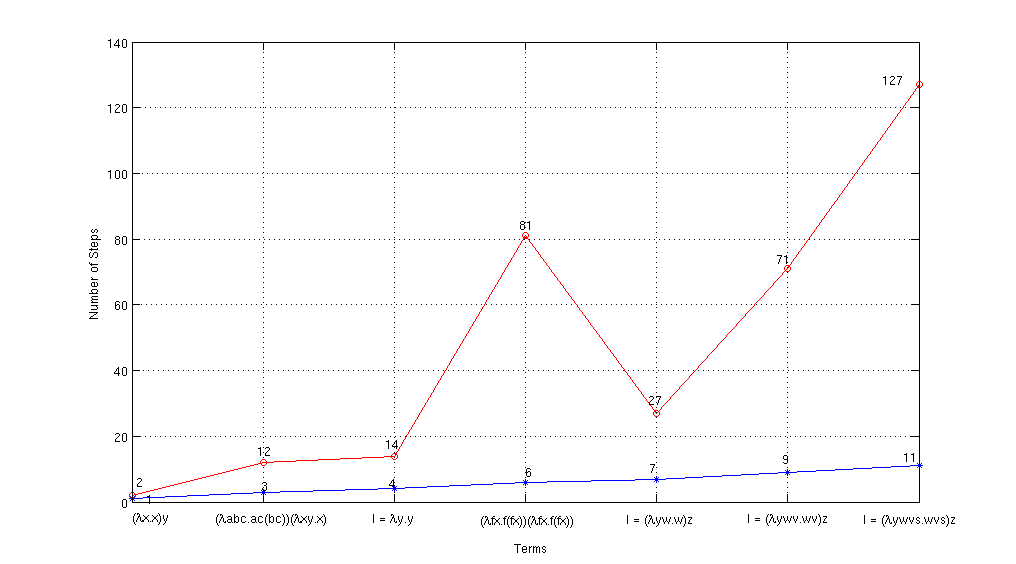
\includegraphics[width=\textwidth]{pics/steps}
\caption{Reduction steps needed for normal reduction and explicit substitution}
\label{fig:termraw}
\end{figure}











